\documentclass[thesis.tex]{subfiles}
\begin{document}

\chapter{Main}\label{chap:basics}

The REAL stuff. All your precious work written down for the benefit of humanity.

\section{Overview}

\section{The meaty Stuff, part 1}

\subsection{The meaty Stuff, part 1.1}

\section{Oh look! Equations!}

\begin{equation}
L(\mathrm{x}, \omega_o) = \sum\limits_{i=1}^{M} f_r(\mathrm{x}, \overrightarrow{\mathrm{x}\mathrm{x}_i}, \omega_o) \cdot G(\mathrm{x}, \mathrm{x}_i) \cdot \hat{V}(\mathrm{x}, \mathrm{x}_i) \cdot I_i(\overrightarrow{\mathrm{x}_i\mathrm{x}})
\end{equation}

\begin{align}
f_r(\mathrm{x}, \overrightarrow{\mathrm{x}\mathrm{x}_i}, \omega_o) =& \frac{\rho_d}{\pi}\\
I_i(\overrightarrow{\mathrm{x}_i\mathrm{x}}) =& \frac{\rho_i}{\pi} \phi_i
\end{align}


\begin{equation} \label{eq:rsmdiffuse}
L_d (\mathrm{x}) = \frac{\rho_d}{\pi} \sum\limits_{i=1}^{M} 
(\hat{\mathbf{n}} \cdot \overrightarrow{\mathrm{x}\mathrm{x}_i} )^+ \cdot
\underbrace{\frac{(\hat{\mathbf{n}}_i\cdot \overrightarrow{\mathrm{x}_i\mathrm{x}})^+}{||\mathrm{x} - \mathrm{x}_i||^2 + A_i} \cdot  \frac{\rho_i}{\pi} \phi_i}_{L_i}
\end{equation}
The diffuse reflectivity $\rho_d$ at the point $\mathrm{x}$ is factored out - it can be applied easily during the cache interpolation stage.

\subsection{Oh look! Images, neatly aligned!}
\begin{figure}[h!]
\centering
\subcaptionbox{Color}{
\begin{subfigure}[b]{0.22\textwidth}

\includegraphics[width=\textwidth]{texture_sample/curtain_color}
\end{subfigure} }
\subcaptionbox{Normalmap}{
\begin{subfigure}[b]{0.22\textwidth}

\includegraphics[width=\textwidth]{texture_sample/curtain_normal}
\end{subfigure} }
\subcaptionbox{Roughness}{
\begin{subfigure}[b]{0.22\textwidth}
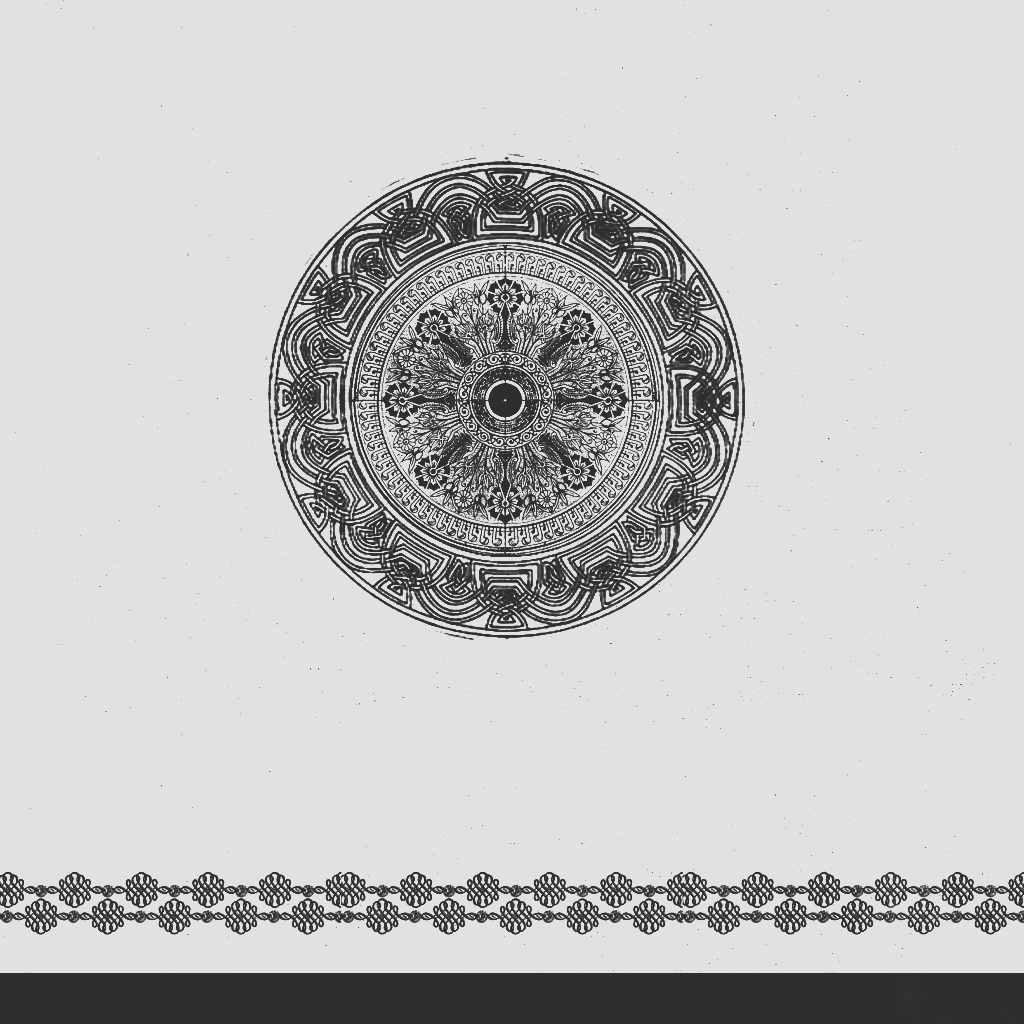
\includegraphics[width=\textwidth]{texture_sample/curtain_roughness}
\end{subfigure} }
\subcaptionbox{Metallic}{
\begin{subfigure}[b]{0.22\textwidth}
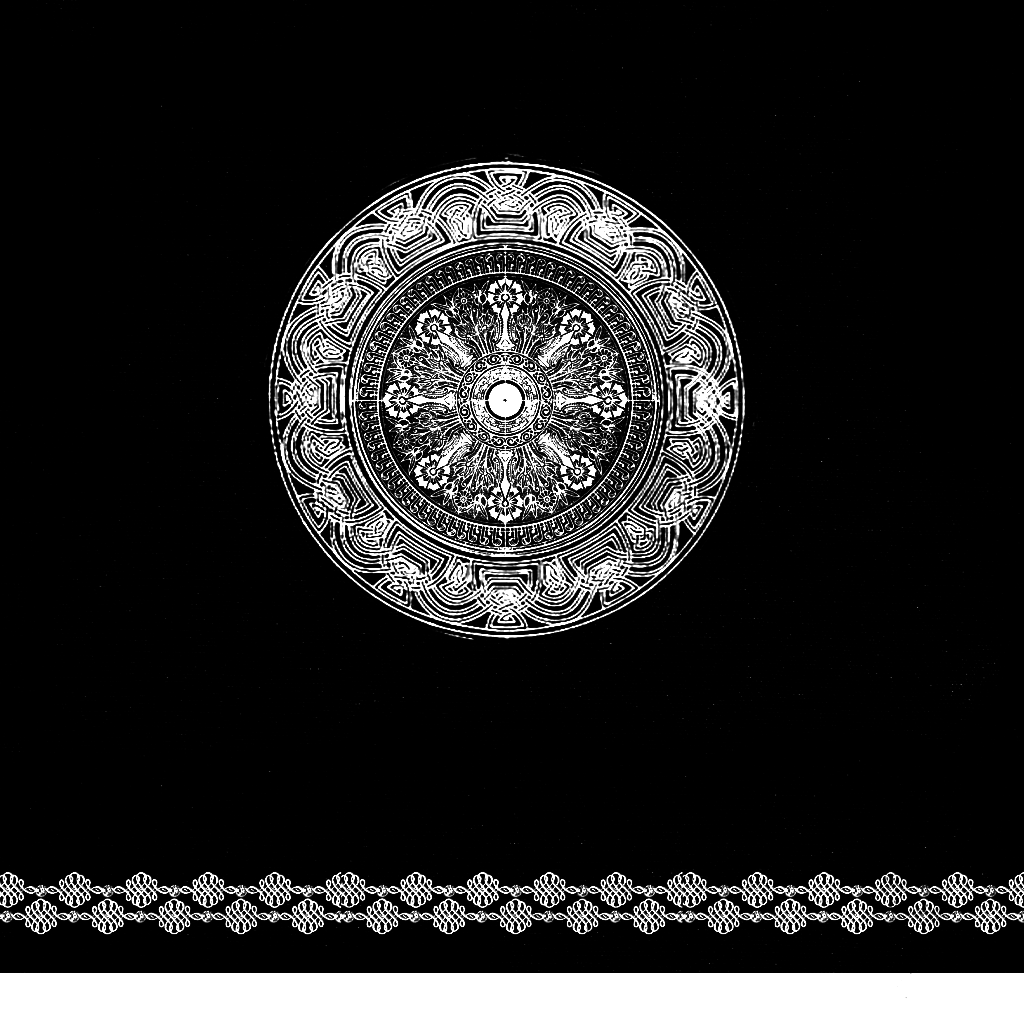
\includegraphics[width=\textwidth]{texture_sample/curtain_metallic}
\end{subfigure} }
\caption{Texture setup demonstrated on curtain from sponza scene.}
\label{fig:texturesample}
\end{figure}

\subsection{Oh look! Code!} \label{sec:impl:cachealloc}


\begin{lstlisting}[language=GLSL]
void mainImage( out vec4 fragColor, in vec2 fragCoord )
{
	vec2 uv = fragCoord.xy / iResolution.xy;
	fragColor = vec4(uv,0.5+0.5*sin(iGlobalTime),1.0);
}
\end{lstlisting}

\subfilebib % Makes bibliography available when compiling as subfile
\end{document}